\chapter{尾侧前额叶皮层:搜寻目标}
尾侧PF皮层有助于通过显性注意力(眼球运动)和隐性注意力对食物和食物迹象等物体进行视觉搜索,它的连接解释了它如何执行这些功能。尾侧PF皮层,包括额眼区(FEF),与视觉皮层的背侧和腹侧流以及脑干动眼神经核都有联系。明显的注意依赖于它与脑干动眼核的连接,直接或间接地通过上丘和基底神经节。隐蔽注意力依赖于增强的感觉反应,这种反应是通过与视觉皮层以及其他感觉区域的相互作用来调节的。在早期灵长类动物中,随着眶侧PF皮层的颗粒状部分,尾侧PF皮层也在进化(第2章)。这两个新区域一起导致了在精细分支生态位的杂乱环境中发现、关注和评估物体的改进。

\section{介绍}
在前一章中,我们认为眶内PF皮层根据当前的生物需求对物体赋值。本章提出,尾侧前额叶皮层搜索这些物体,它是通过隐蔽地注意周围目标和将眼睛朝向这些目标来实现的。本章的大部分内容都是关于视觉和眼球运动的,它们在脊椎动物历史的早期就已经进化出来了。眼睛和眼外肌肉的证据出现在最古老的脊椎动物和前脊椎动物化石中,有些可以追溯到500多年前(Shu等 2003)。但是灵长类动物在视觉和眼球运动方面有一些重要的创新,比如发展出了中央凹和三色视觉(第2章)。如果我们正确地认为,尾侧PF皮层首先出现在早期灵长类动物身上,那么它比中央凹和全彩视觉都要早:这是关于其功能的重要线索。为了理解尾侧PF皮层,我们首先需要看看它的连接是如何允许灵长类的PF皮层使用眼球运动和隐蔽注意力来搜索食物等物体的。
\section{区域}
在猕猴中,尾侧前额叶皮层指的是位于弓状沟膝侧的皮层。图5.1描绘了它的位置。
% TODO: \usepackage{graphicx} required
\begin{figure}
	\centering
	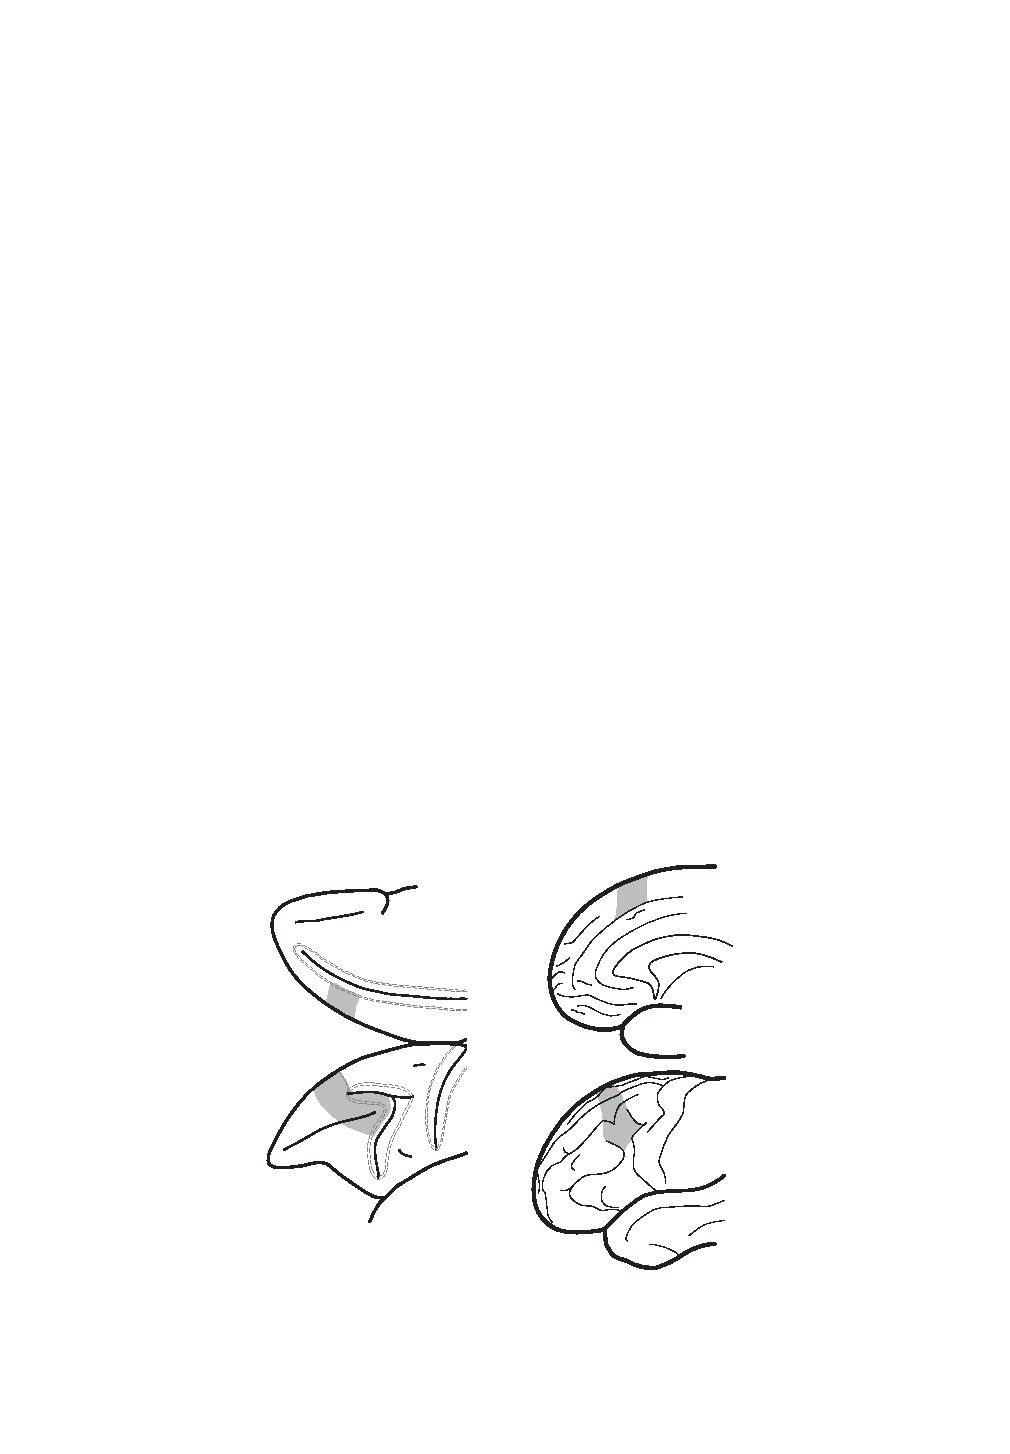
\includegraphics[width=0.7\linewidth]{image_pfc/Fig_5_1}
	\caption{猕猴(左)和人类(右)的尾侧PF皮层。格式如图1.2所示。}
	\label{fig:fig}
\end{figure}

正如我们所定义的那样,尾侧PF皮层总是包括第8区,为了本章的目的,它还包括猕猴主沟的尾侧部分。我们通过注意到,正如在第8区域(Chafee和Goldman-Rakic 1998),主沟尾部的大多数细胞调节其活动与眼球运动相关(Tanila等 1993)来证明这一分组是正确的。Petrides和Pandya(1999)发现了一个位于主沟尾端附近的区域,他们称之为9/46,他们将该区域与相邻的吻侧中外侧PF皮层(46区)和背内侧9区区分开来。顾名思义,Petrides和Pandya认为9/46区具有与9区和46区相似的细胞结构特性,并且这三个区域都具有颗粒状的细胞结构。我们称主沟尾侧皮层为后外侧PF皮层(图1.4),目前将其包括在PF尾侧皮层中。然而,我们承认,在不违反任何解剖学原理的情况下,可以将其包括在PF皮层背侧(第6章)。表1.2使用一个查询标记(“?”)来表示这两个选项。因此,关于后外侧前额叶皮层的许多观点都适用于本章和下一章。

在猕猴中,通过微刺激弓状沟靠近主沟尾端的吻侧岸,可以诱发眼跳运动(Bruce等 1985),这一特性定义了额眼场(FEF)。更高的电流可以通过电流传播,从更大的区域唤起跳视(Robinson和Fuchs 1969),但人们普遍认为低阈值区域对应于FEF。因此,区域8包括FEF,它从典型的颗粒状细胞结构向非颗粒状细胞结构变化(Stanton等 1989)。

Amiez和Petrides(2009)回顾了通过电刺激在人脑中定位FEF的研究。来自中央前上沟吻侧的低阈值刺激,以及来自中央前上沟上方的低阈值刺激,可以诱发眼跳。Amiez等人(2006)使用成像方法来定位与个体受试者皮层解剖相关的激活峰值。FEF,按照这样的定义,始终位于中央前上沟的腹侧分支,这个位置与电刺激所定义的位置大致一致。Amiez和Petrides(2009)提供了猕猴和人类的地图,并表明在这两种情况下,FEF都可以与运动前皮层区分开来,电刺激也可以唤起眼球运动。

微刺激还在猕猴的额叶中发现了第二个眼场:补充眼场(SEF) (Schlag和Schlag- rey 1987)。与FEF一样,SEF中的细胞在扫视前增加活动(Hanes等 1995)。在猕猴中,SEF位于背内侧额叶皮层的第6区(Schlag 和 Schlag- rey 1987;Olson和Gettner 1999),它在人脑中有类似的位置(Amiez和Petrides 2009)。
\section{连接}
图5.2显示了猕猴的尾侧PF皮层的皮质连接,包括FEF。这些数据主要来自Petrides和Pandya(1999),他们将示踪剂注入区域8的细分(区域8B、8Ad或8Av),并描述了它们之间的联系。这项研究比早期的研究更有优势(Petrides和Pandya 1984;Barbas 1988;Barbas 和 Pandya 1989;Cavada和Goldman-Rakic 1989), Petrides和Pandya(1999)进行了小规模和相对选择性的注射。
% TODO: \usepackage{graphicx} required
\begin{figure}
	\centering
	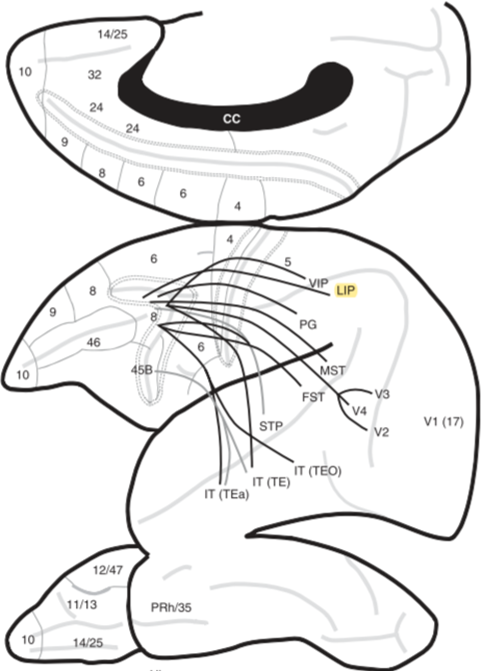
\includegraphics[width=0.7\linewidth]{image_pfc/Fig_5_2}
	\caption{末梢PF皮层的选定连接。图1.4和1.5给出了沟和区域的名称。这些线连接了一些与尾侧PF皮质有轴突直接连接的区域,除非另有说明,假设是相互的。}
	\label{fig:fig}
\end{figure}


根据连接得到以下结论:

\begin{enumerate}
	\item 8Ad区、8B区和后外侧PF皮层与执行眼肌运动和视觉空间功能的区域相连。例如,它们与位于顶骨内沟的LIP区有联系(Cavada和Goldman-Rakic 1989;Andersen等 1990), LIP中的细胞编码眼球运动(Snyder等 1997)。同样的PF区域与下顶叶皮层的PG区域有连接(Cavada和Goldman-Rakic 1989),该区域的许多细胞编码眼睛方向(Sakata等 1980)。最后,8Ad区与颞区MST区有联系,在MST区,细胞对视觉刺激的运动做出反应Celebrini和Newsome 1995)。
	\item 这些视觉区域构成了背侧视觉流的一部分(Ungerleider和Mishkin 1982;Milner和Goodale 2007),以区别于腹侧视觉流。一般来说,背侧流包括后顶叶区域,处理有关动作空间目标的信息,腹侧流包括颞下区域,处理有关视觉刺激的颜色、形状和纹理的信息。
	\item FEF接收早期(低阶)视觉区域的信息,如枕部视觉区V2和V3 (Stanton et al. 1995),但8Ad区和后外侧PF皮层不接收信息。因此,FEF接收到的高度处理视觉信息比PF皮层尾端的其他部分和PF皮层的其他部分要少。
	\item 8Av区不同于8Ad区、8B区和后外侧PF区,分别与腹侧流和背侧流有联系。8Av区与TEO区有联系(Webster et al. 1994),也与颞下皮层的其他部分有联系,如颞上沟下岸的皮层(Petrides和Pandya 1999)。
	\item 尾侧PF皮层各组成区域之间相互连接紧密。8Ad区和8Av区彼此相互投射,并与后外侧PF皮层(9/46区)相互投射。这些相互联系支持我们将后外侧皮层纳入本章。如图1.8所示,我们所定义的尾侧PF皮层与Price和Drevets(2010)所定义的尾侧网络非常相似。
\end{enumerate}

图5.2和前面的列表涉及皮质连接,但尾侧PF皮质的皮质连接也解释了其功能的一些重要内容:

\begin{enumerate}
	\item FEF (Künzle, 1976;Huerta et al. 1986)、8区其余部分(Fries 1984)和后外侧PF皮层(Selemon和Goldman-Rakic 1988)都向上丘发送直接投影。在所有脊椎动物中,上丘及其同源体都有定位头部感受器的功能。因此,这些皮质连接指向了尾侧PF皮层在控制眼球运动方面的作用,但大脑皮层的许多其他部分也投射到上丘(Leichnetz等 1981;Fries 1984),所以这种解剖特征并不能将PF皮层与其他区域区分开来。
	\item FEF还可以通过向基底神经节的投射影响上丘的活动。FEF投射到尾状核的内侧(Stanton等 1988),后者又投射到黑质网状部(Hedreen和DeLong 1991)。该核投射到上丘,在那里发挥抑制作用(Hikosaka和Wurtz 1985)。
	\item 最后,FEF直接投射到脑干动眼肌核(Segraves 1992;Yan等 2001)。
\end{enumerate}

\subsection{总结}
尾侧PF皮层的连接指纹表明,它接受直接的、较低的视觉输入,它具有与背侧和腹侧视觉蒸汽平行的背侧-腹侧区别,并且它通过基底神经节到上丘的投射直接或间接地输出到动眼神经核

\section{指纹}

\subsection{损伤和激活}

\subsection{损伤和活动}

\subsection{活动和激活}



\subsection{结论}